\documentclass[man]{apa6}

\usepackage{amssymb,amsmath}
\usepackage{ifxetex,ifluatex}
\usepackage{fixltx2e} % provides \textsubscript
\ifnum 0\ifxetex 1\fi\ifluatex 1\fi=0 % if pdftex
  \usepackage[T1]{fontenc}
  \usepackage[utf8]{inputenc}
\else % if luatex or xelatex
  \ifxetex
    \usepackage{mathspec}
    \usepackage{xltxtra,xunicode}
  \else
    \usepackage{fontspec}
  \fi
  \defaultfontfeatures{Mapping=tex-text,Scale=MatchLowercase}
  \newcommand{\euro}{€}
\fi
% use upquote if available, for straight quotes in verbatim environments
\IfFileExists{upquote.sty}{\usepackage{upquote}}{}
% use microtype if available
\IfFileExists{microtype.sty}{\usepackage{microtype}}{}

% Table formatting
\usepackage{longtable, booktabs}
\usepackage{lscape}
% \usepackage[counterclockwise]{rotating}   % Landscape page setup for large tables
\usepackage{multirow}		% Table styling
\usepackage{tabularx}		% Control Column width
\usepackage[flushleft]{threeparttable}	% Allows for three part tables with a specified notes section
\usepackage{threeparttablex}            % Lets threeparttable work with longtable

% Create new environments so endfloat can handle them
% \newenvironment{ltable}
%   {\begin{landscape}\begin{center}\begin{threeparttable}}
%   {\end{threeparttable}\end{center}\end{landscape}}

\newenvironment{lltable}
  {\begin{landscape}\begin{center}\begin{ThreePartTable}}
  {\end{ThreePartTable}\end{center}\end{landscape}}

  \usepackage{ifthen} % Only add declarations when endfloat package is loaded
  \ifthenelse{\equal{\string man}{\string man}}{%
   \DeclareDelayedFloatFlavor{ThreePartTable}{table} % Make endfloat play with longtable
   % \DeclareDelayedFloatFlavor{ltable}{table} % Make endfloat play with lscape
   \DeclareDelayedFloatFlavor{lltable}{table} % Make endfloat play with lscape & longtable
  }{}%



% The following enables adjusting longtable caption width to table width
% Solution found at http://golatex.de/longtable-mit-caption-so-breit-wie-die-tabelle-t15767.html
\makeatletter
\newcommand\LastLTentrywidth{1em}
\newlength\longtablewidth
\setlength{\longtablewidth}{1in}
\newcommand\getlongtablewidth{%
 \begingroup
  \ifcsname LT@\roman{LT@tables}\endcsname
  \global\longtablewidth=0pt
  \renewcommand\LT@entry[2]{\global\advance\longtablewidth by ##2\relax\gdef\LastLTentrywidth{##2}}%
  \@nameuse{LT@\roman{LT@tables}}%
  \fi
\endgroup}


  \usepackage{graphicx}
  \makeatletter
  \def\maxwidth{\ifdim\Gin@nat@width>\linewidth\linewidth\else\Gin@nat@width\fi}
  \def\maxheight{\ifdim\Gin@nat@height>\textheight\textheight\else\Gin@nat@height\fi}
  \makeatother
  % Scale images if necessary, so that they will not overflow the page
  % margins by default, and it is still possible to overwrite the defaults
  % using explicit options in \includegraphics[width, height, ...]{}
  \setkeys{Gin}{width=\maxwidth,height=\maxheight,keepaspectratio}
\ifxetex
  \usepackage[setpagesize=false, % page size defined by xetex
              unicode=false, % unicode breaks when used with xetex
              xetex]{hyperref}
\else
  \usepackage[unicode=true]{hyperref}
\fi
\hypersetup{breaklinks=true,
            pdfauthor={},
            pdftitle={Child language experience in a Tseltal Mayan village},
            colorlinks=true,
            citecolor=blue,
            urlcolor=blue,
            linkcolor=black,
            pdfborder={0 0 0}}
\urlstyle{same}  % don't use monospace font for urls

\setlength{\parindent}{0pt}
%\setlength{\parskip}{0pt plus 0pt minus 0pt}

\setlength{\emergencystretch}{3em}  % prevent overfull lines


% Manuscript styling
\captionsetup{font=singlespacing,justification=justified}
\usepackage{csquotes}
\usepackage{upgreek}

 % Line numbering
  \usepackage{lineno}
  \linenumbers


\usepackage{tikz} % Variable definition to generate author note

% fix for \tightlist problem in pandoc 1.14
\providecommand{\tightlist}{%
  \setlength{\itemsep}{0pt}\setlength{\parskip}{0pt}}

% Essential manuscript parts
  \title{Child language experience in a Tseltal Mayan village}

  \shorttitle{Child language experience in a Tseltal Mayan village}


  \author{Marisa Casillas\textsuperscript{1}, Penelope Brown\textsuperscript{1}, \& Stephen C. Levinson\textsuperscript{1}}

  % \def\affdep{{"", "", ""}}%
  % \def\affcity{{"", "", ""}}%

  \affiliation{
    \vspace{0.5cm}
          \textsuperscript{1} Max Planck Institute for Psycholinguistics  }

  \authornote{
    Correspondence concerning this article should be addressed to Marisa
    Casillas, Wundtlaan 1, 6525 XD Nijmegen, The Netherlands. E-mail:
    \href{mailto:Marisa.Casillas@mpi.nl}{\nolinkurl{Marisa.Casillas@mpi.nl}}
  }


  \abstract{Enter abstract here. Each new line herein must be indented, like this
line.}
  \keywords{keywords \\

    \indent Word count: X
  }





\usepackage{amsthm}
\newtheorem{theorem}{Theorem}[section]
\newtheorem{lemma}{Lemma}[section]
\theoremstyle{definition}
\newtheorem{definition}{Definition}[section]
\newtheorem{corollary}{Corollary}[section]
\newtheorem{proposition}{Proposition}[section]
\theoremstyle{definition}
\newtheorem{example}{Example}[section]
\theoremstyle{definition}
\newtheorem{exercise}{Exercise}[section]
\theoremstyle{remark}
\newtheorem*{remark}{Remark}
\newtheorem*{solution}{Solution}
\begin{document}

\maketitle

\setcounter{secnumdepth}{0}



\section{Introduction}\label{introduction}

A great deal of work in developmental language science revolves around
one central question: What linguistic evidence (i.e., what types and how
much) is needed to support first language acquisition? In pursuing this
topic, many researchers have fixed their sights on child-directed speech
(CDS), showing that it is linguistically distinctive
(REFS)\textbf{{[}TASK 00: Add missing references{]}}, interactionally
rich (REFS), preferred by infants (REFS), and---perhaps most
importantly---facilitates word learning (REFS). One might then conclude
that CDS is an essential component for acquiring a first language. Yet
ethnographic reports from a number of traditional, non-Western
communities suggest that children easily acquire their community's
language(s) with little or no CDS (REFS). If so, CDS may not be
essential for learning language; just useful for facilitating certain
aspects of language development. In this paper we investigate the
language environment and early development of 10 Tseltal Mayan children
growing up in a community that reportedly uses very little CDS with
infants and young children (REFS Brown).

\subsection{Child-directed speech}\label{child-directed-speech}

The amount of CDS children hear influences their language development,
particularly their vocabulary (REFS). For example, \textbf{{[}TASK 01:
Add examples of input-vocab link{]}}. CDS has also been linked to young
children's speed of lexical retrieval (REFS Weisleder; LuCiD) and
syntactic development (REFS Huttenlocher). \textbf{{[}TASK 02: Read
Huttenlocher and add details here{]}}. The conclusion drawn from much of
this work is that CDS is an ideal register for learning
words---especially concrete nouns and verbs---because it is tailored to
maximize a child's moment-to-moment interest and understanding (REFS).
Indeed, even outside of first-person interaction, infants and young
children prefer listening to CDS over adult-directed speech (REFS
ManyBabies, etc.), suggesting that CDS is useful in catching,
maintaining, and focusing children's attention. There are, however, a
few significant caveats to the body of work relating CDS quantity to
language development.

First, while there is overwhelming evidence linking CDS quantity to
vocabulary size, links to grammatical development are more scant (REFS:
Huttenlocher; Frank et al.). Children must master the systemic
underpinnings of their language(s), e.g., the phonology, morphology, and
syntax. While the advantage of CDS for referential word learning is
clear, it is less obvious how CDS facilitates syntactic learning.
\textbf{{[}TASK 03: Add argument from Yurovsky paper + refrences
therein{]}} On the other hand, there is a wealth of evidence that both
children and adults' syntactic knowledge is highly lexically specified
(REFS), and that, crosslinguistically, children's vocabulary size is one
of the most robust predictors of their early syntactic development
(REFS). In short, what is good for the lexicon may also be good for
syntax. For now, however, the link between CDS and other aspects of
grammatical development still needs to be more thoroughly tested.

Second, \textbf{{[}TASK 04: Add paragraph on burstiness{]}}

Third, prior work has typically focused on Western (primarily North
American) populations, limiting our ability to generalize these effects
to children acquiring language worldwide (REFS: WEIRD; Lieven, 1994).
While we do gain valuable insight by looking at \emph{within-population}
variation (e.g., REFS), we can more effectively find places where our
assumptions break down by studying \emph{new} populations. Linguistic
anthropologists working in non-Western communities have long reported
that caregiver interaction styles vary immensely from place to place,
with some caregivers using little or no CDS to young children (REFS
Gaskins, 2006). Children in these communities reportedly acquire
language with `typical'-looking benchmarks. For example, they start
pointing (REFS Liszkowski) and talking (REFS Rogoff et al., 2003?;
Brown??) around the same time we would expect for Western middle-class
infants. If indeed these children acquire language without delay despite
little or no CDS, it forces us to reconsider what kind of linguistic
evidence is necessary for children to learn language.

\subsection{Language development in non-WEIRD
communities}\label{language-development-in-non-weird-communities}

To our knowledge, only a handful of researchers have used methods from
developmental psycholinguistics to describe the language environments
and linguistic development of children growing up in traditional,
non-Western communities. We focus here on \emph{quantitative} language
development measures because the key claims about CDS and linguistic
development are themselves quantitative in nature. We briefly highlight
two recent efforts along these lines, but see Cristia et al. (2017) for
a recent review.

Scaff, Cristia, and colleagues (REFS 2017; in preparation) have used a
number of methods to estimate how much speech children hear in a
Tsimane' forager-horticulturalist population in the Bolivian lowlands.
Their daylong recordings show that Tsimane' children between 0;6 and 6;0
hear around 5 minutes of CDS per hour, with no evidence of age-related
change. For comparison, children from North American homes between 0;3
and 3;0 are estimated to hear around 11 minutes of CDS per hour in
daylong recordings (REFS: Bergelson, Casillas, et al., see also REFS the
newer Tamis-LeMonda paper; maybe give estimates w/ age ranges for
each??). Tsimane' children also heard \textasciitilde{}10 minutes of
other-directed speech per hour (e.g., talk between adults)---more than
the \textasciitilde{}7 minutes of adult-directed speech per hour
estimated for North American homes (REFS Bergelson, Casillas, et al.).
The additional other-directed speech may be attributable to the fact
that the Tsimane' live in extended family clusters of 3--4 households;
speakers are typically in close proximity to 5--8 others (REFS Cristia
et al., 2017).

Laura Shneidman and colleagues (REFS; 2010; 2012) analyzed speech from
1-hour at-home video recordings of Yucatec Mayan children and American
children between 13 and 35 months. Shneidman and Goldin-Meadow's (REFS;
2012) analyses of the video recordings yielded four main findings:
compared to the American children, (a) the Mayan children heard many
fewer utterances per hour, (b) a much smaller proportion of the
utterances they heard were \emph{child-directed}, (c) the proportion of
child-directed utterances increased dramatically with age, matching
American children's by 35 months, and that (d) most of the added CDS
came from other children (e.g., older siblings and cousins). They also
demonstrated that the lexical diversity of CDS children heard at 24
months---particularly from adult speakers---predicted their vocabulary
knowledge at 35 months.

These groundbreaking studies on Tsimane and Yucatec Mayan children's
early language environments lead us to a number of important interim
conclusions. First, children in each of these communities appear able to
acquire their languages with relatively little CDS. Second, the
frequency with which they are addressed increases with age. Third, other
children may be the primary source of CDS in similar communities. And
finally, despite these differences, CDS from adults may still be the
most robust predictor of vocabulary growth.

\subsection{The current study}\label{the-current-study}

We examine the early langage experience of 10 Tseltal Mayan children
under age 3;0. Similar to previous work by Shneidman, Scaff, Cristia,
and colleages, we aimed to estimate how much speech children overheard,
how much was directed to them, and how those quantities changed with
age. To this we add new sampling techniques in order to present a more
nuanced view of what counts in children's linguistic `input'. We also
present evidence on the vocal maturity children's early productions and
discuss how it is influenced (and not influenced) by CDS.

We chose to investigate the early language environments of Tseltal Mayan
children because prior ethnographic work (REFS: Brown??) suggests that,
as in other traditional Mayan communities, caregivers infrequently speak
directly to children, but that children nonetheless develop linguistic
skills without any apparent delay. The children in our dataset come from
a linguistically and culturally similar community to that in Shneidman's
(REFS: 2010 + add other stuff that's not nec lg) work, which allows us
to compare differences between the two in early language experience and
development more directly than previous work on non-WEIRD communities
(see Pye REFS and the comparative ethnographic work previously done on
this cultural family: REFS). We provide more details on this community
and the corpus of data analyzed in the \emph{Methods}.

Finally, a major contribution of this work is the use of daylong
recordings to estimate the quantity and types of speech that children
hear over the course of a day at home. Using a novel combination of a
lightweight audio recorder and wearable photo camera, we were able to
track children's movements and interactions over the course of a
9--11-hour period in which the experimenter was not present. With
long-format recordings of this kind we can make precise descriptive
estimates about the speech children hear: typical quantities, variation
within a day, and more (REFS: see also Tamis-LeMonda et al\ldots{}.).

Our aim in this paper is to develop a nuanced child language environment
profile for Tseltal Mayan. In line with prior work, we predicted that
Tseltal Mayan children hear little CDS, that the amount of CDS increases
with age, that most CDS comes from other children, and that, despite
this, Tseltal Mayan children would hit early speech production
benchmarks on par with Western children. We additionally predicted that
children's language environment would be bursty---that brief,
high-intensity interactions would be sparsely distributed throughout the
day, accounting for the majority of children's daily CDS---and that
children's responsiveness and vocal maturity would be maximized during
these moments of high-intensity interaction.

\section{Methods}\label{methods}

\subsection{How to define temporal contingency for turn
taking}\label{how-to-define-temporal-contingency-for-turn-taking}

Many other studies of child-caregiver turn taking use an arbitrary
cut-off for detecting contingency (5 seconds?? Look up references). We
base ours on measures of turn taking in interactions with infants and
young children. Hilbrink et al. (2015) looked at interaction in a
longitudinal corpus from 3 to 18 months and found that infants'
responses to mothers began between -700ms and 1200ms relative to the end
of the mothers' turns. Complementarily, mothers' responses to infant
vocalizations began between -350ms and 650ms relative to the end of the
infants' turns. Casillas et al. (2016) investigated the timing of
question-answer responses from caregiver to child and from child to
caregiver with children between 20 and 35 months. In their study,
children's responses typically started between -500ms and 650ms relative
to the end of their caregivers' turns. Caregivers' responses typically
started between -1000ms and 400ms relative to the end of their
children's turns. Because both studies focused on fairly intensive bouts
of interaction, and both within WEIRD parental contexts, we defined
contingent responses in the current data with slightly generous
allowances for overlap and gap: contingent responses must begin with no
more than 1000ms of overlap and 2000ms of gap relative to the offset of
the first speaker's turn. We used this same criteria for finding
child-to-other turn transitions and other-to-child turn transitions.
Transitions were only counted if the other speaker's turn was coded as
addressed to \enquote{T} (the target child).

\subsection{Participants}\label{participants}

\subsection{Material}\label{material}

\subsection{Procedure}\label{procedure}

\subsection{Data analysis}\label{data-analysis}

\section{Results}\label{results}

\subsection{Still to graph}\label{still-to-graph}

3: sliding window in random to match mean TDS rate/TT transition rates
4: utt length, repetitiveness, F0 peaks and ranges

\subsection{SHOULD I ADD DATAPOINTS ON THE UPH FIGS TO SHOW SHNEIDMAN'S
DATA?}\label{should-i-add-datapoints-on-the-uph-figs-to-show-shneidmans-data}

Age 1: - US: CDS 616 (SD=231); ADS/OCDS 278 (SD=247) -- 79\% XDS from
MOT (\textasciitilde{}60\% XDS MOT is CDS); 8\% XDS from children
(mostly ADS/OCDS) - Mayan: CDS 86 (SD=59); ADS/OCDS 342 (SD=201) -- 31\%
XDS from MOT (\textasciitilde{}4\% XDS MOT is CDS); 60\% XDS from
children (\textasciitilde{}50\% XDS other kids was ADS/OCDS) Age18mo?:
Age 2: - US: CDS M=815, SD=376; ADS/OCDS M=411, SD=318 -- M=65\%,
SD=28\% from MOT (directed: M=800, SD=381; overheard: M=211, SD =55); --
M=7\%, SD=10\% from kids (directed: M=15, SD=22; overheard: M=86,
SD=141) - Mayan: CDS M=274, SD=166; ADS/OCDS M=271, SD=136 -- M=19\%,
SD=17\% from MOT (directed:M=104, SD=100; overheard:M=82 SD=52); --
M=61\%, SD=27\% from kids (directed:M=104, SD=100; overheard:M=82 SD=52)
Age35mo?

\subsubsection{Observation only data}\label{observation-only-data}

13 months Directed speech 140 (55); Overheard speech 377 (176) 18 months
Directed speech 211 (70); Overheard speech 240 (96) 24 months Directed
speech 315 (69); Overheard speech 360 (73) (I think these data weren't
coded for adult vs.~child speaker)

\begin{figure}
\centering
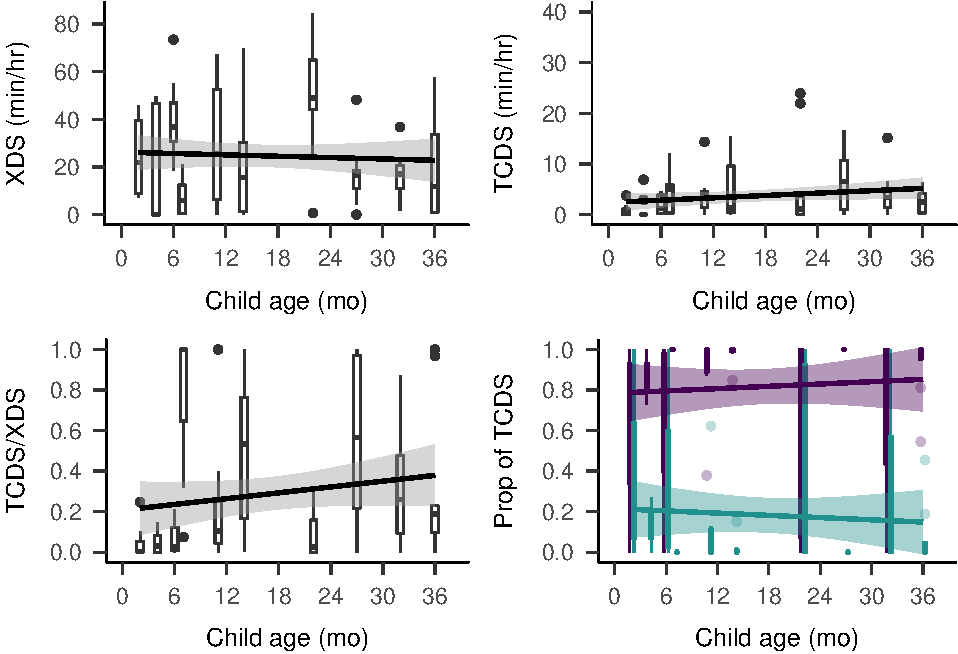
\includegraphics{Tseltal-CLE_files/figure-latex/plot_XDS_TDS_quantity_random-1.pdf}
\caption{}
\end{figure}

\begin{figure}
\centering
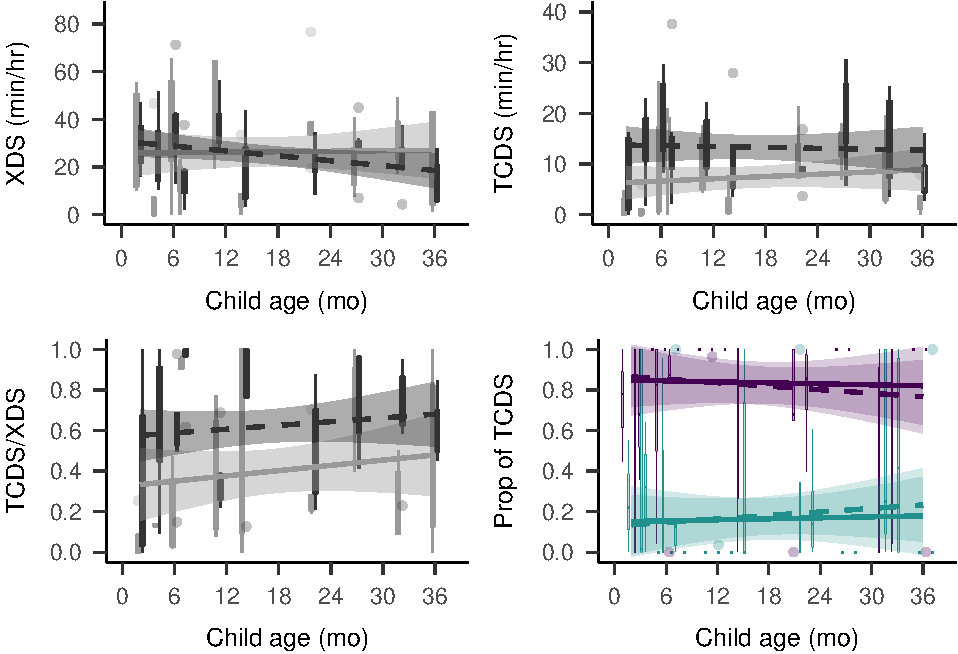
\includegraphics{Tseltal-CLE_files/figure-latex/plot_XDS_TDS_quantity_nonrandom-1.pdf}
\caption{}
\end{figure}

\begin{figure}
\centering
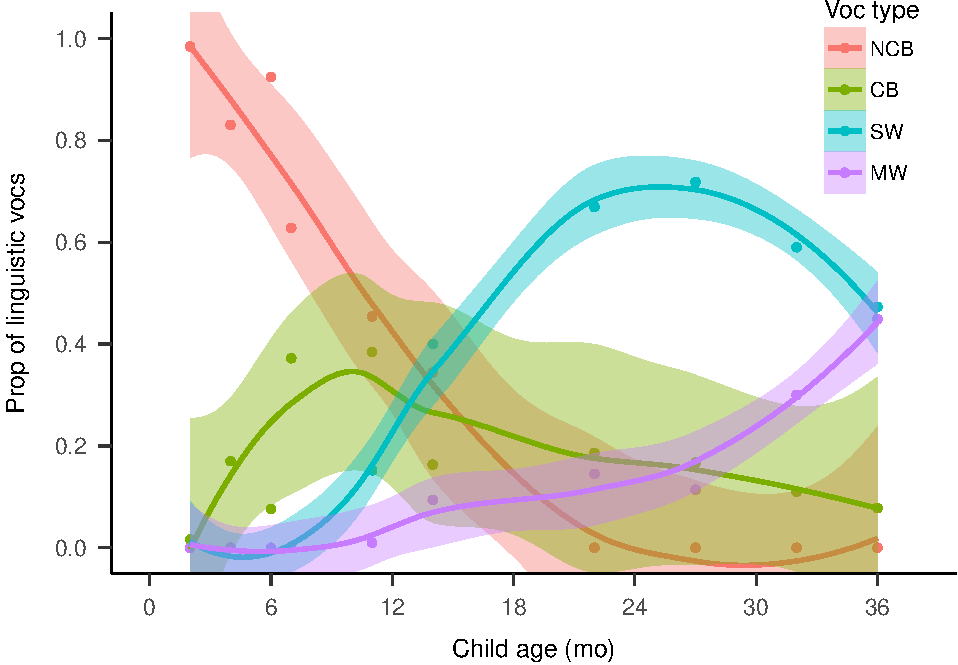
\includegraphics{Tseltal-CLE_files/figure-latex/plot_chi_voctypes_overall-1.pdf}
\caption{}
\end{figure}

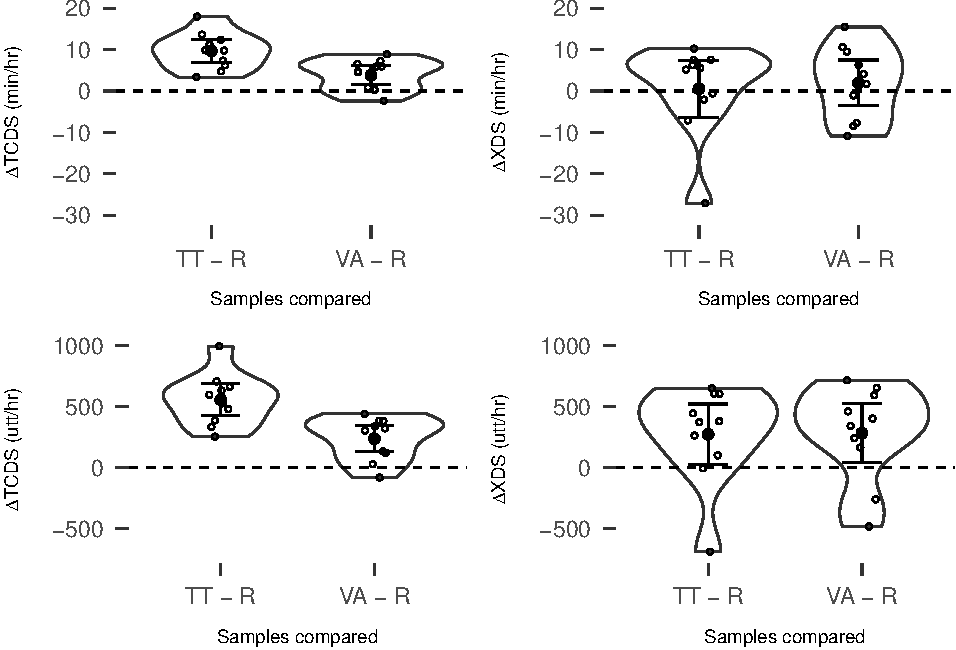
\includegraphics{Tseltal-CLE_files/figure-latex/plot_sample_differences-1.pdf}
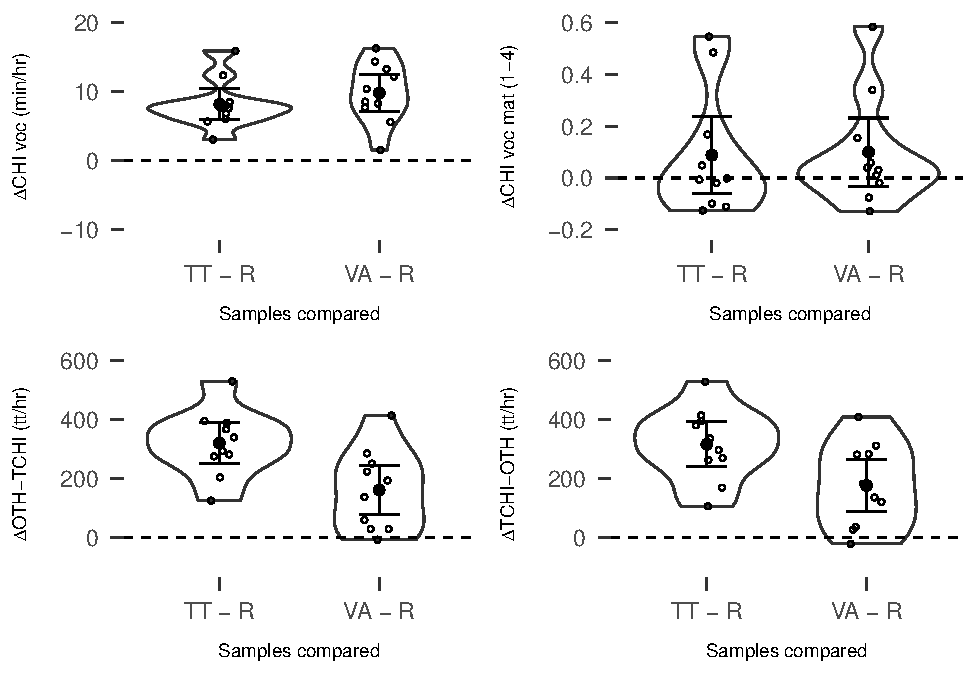
\includegraphics{Tseltal-CLE_files/figure-latex/plot_sample_differences-2.pdf}

\section{Discussion}\label{discussion}

\newpage

\section{References}\label{references}

\begingroup
\setlength{\parindent}{-0.5in} \setlength{\leftskip}{0.5in}

\hypertarget{refs}{}

\endgroup






\end{document}
